% Unofficial University of Cambridge Poster Template
% https://github.com/andiac/gemini-cam
% a fork of https://github.com/anishathalye/gemini
% also refer to https://github.com/k4rtik/uchicago-poster
% Use LuaLaTeX
% refer to 
% https://www.overleaf.com/latex/templates/modelo-de-poster-ppgca-utfpr/crxjybcnyrfq

\documentclass[final]{beamer}
% \documentclass[final,8pt]{beamer}
% \documentclass[final,20pt]{beamer}

% ====================
% Packages
% ====================

\usepackage[T1]{fontenc}
\usepackage{lmodern}
\usepackage[orientation=portrait,size=a0,scale=1.3]{beamerposter}
% \usetheme{gemini}
\usetheme{noctchill}
% \usecolortheme{gemini}
% \usecolortheme{mit}
% \usecolortheme{labsix}
% \usecolortheme{nott}
\usecolortheme{noctchill}
\usepackage{graphicx}
\usepackage{booktabs}
\usepackage{tikz}
\usepackage{pgfplots}
\pgfplotsset{compat=1.14}
\usepackage{anyfontsize}
\usepackage{lipsum}
\usepackage{ragged2e}
\renewcommand{\raggedright}{\leftskip=0pt \rightskip=0pt plus 0cm}


% ====================
% Lengths
% ====================

% If you have N columns, choose \sepwidth and \colwidth such that
% (N+1)*\sepwidth + N*\colwidth = \paperwidth
\newlength{\sepwidth}
\newlength{\colwidth}
\setlength{\sepwidth}{0.033\paperwidth}
\setlength{\colwidth}{0.45\paperwidth}
% \setlength{\sepwidth}{0.025\paperwidth}
% \setlength{\colwidth}{0.3\paperwidth}

\newcommand{\separatorcolumn}{\begin{column}{\sepwidth}\end{column}}

% ====================
% Title
% ====================

\title{Leveraging Parameter-Efficient Fine-Tuning for Multilingual Abstractive Summarization}

\author{Jialun Shen \inst{1} \and Yusong Wang$^*$ \inst{1,2}}

\institute[shortinst]{\inst{1} Tokyo Institute of Technology \samelineand \inst{2} Guangdong Institute of Intelligence Science and Technology}

% ====================
% Footer (optional)
% ====================

% \footercontent{
%   \href{https://utfpr.edu.br/ct/ppgca}{utfpr.edu.br/ct/ppgca} \hfill
%   Mostra de Trabalhos do PPGCA --- TechTalks 2024 \hfill
%   \href{mailto:ppgca-ct@utfpr.edu.br}{ppgca-ct@utfpr.edu.br}}
\footercontent{
  \href{https://github.com/sgallon-rin/peft-mas}{github.com/sgallon-rin/peft-mas} \hfill
  % The 13th CCF International Conference on Natural Language Processing and Chinese Computing (NLPCC 2024) \hfill
  The 13th CCF International Conference on Natural Language Processing and Chinese Computing \hfill
  \href{mailto:wangyusong@gdiist.cn}{wangyusong@gdiist.cn}}
% (can be left out to remove footer)


% ====================
% Logo (optional)
% ====================

% use this to include logos on the left and/or right side of the header:
\logoleft{
\includegraphics[height=8cm]{logos/titech-logo.png}}
\logoright{
\includegraphics[height=8cm]{logos/gdiist-logo.png}}
% \logoleft{\hspace{20ex}
\includegraphics[height=7.5cm]{logos/titech-logo.png}}

% ====================
% Body
% ====================

\begin{document}

\raggedright

\begin{frame}[t]
\begin{columns}[t]
\separatorcolumn

\begin{column}{\colwidth}

  \begin{alertblock}{Motivation}

    \begin{itemize}
      \item Full fine-tuning of \textbf{Pre-trained Language Models (PLMs)} is \textbf{computationally expensive} and \textbf{resource-intensive}.
      As the demand for \textbf{multilingual NLP} grows, the need for efficient and scalable transfer learning methods becomes critical to make PLMs practical for real-world use in diverse linguistic settings.
      \item \textbf{Parameter-Efficient Fine-Tuning (PEFT)} methods like \textbf{Prefix-tuning} and \textbf{LoRA} have shown potential in reducing the number of parameters updated while retaining performance in monolingual tasks.
      However, \textbf{their effectiveness in multilingual tasks remains underexplored}.
      \item \textbf{Key Contribution}: We are the first to systematically evaluate PEFT methods in \textbf{multilingual abstractive summarization}, demonstrating clear \textbf{efficiency-performance trade-offs}.
      Our work sets new \textbf{benchmarks} for advancing \textbf{efficient multilingual NLP}.
    \end{itemize}

  \end{alertblock}

  \begin{figure}
    \centering
    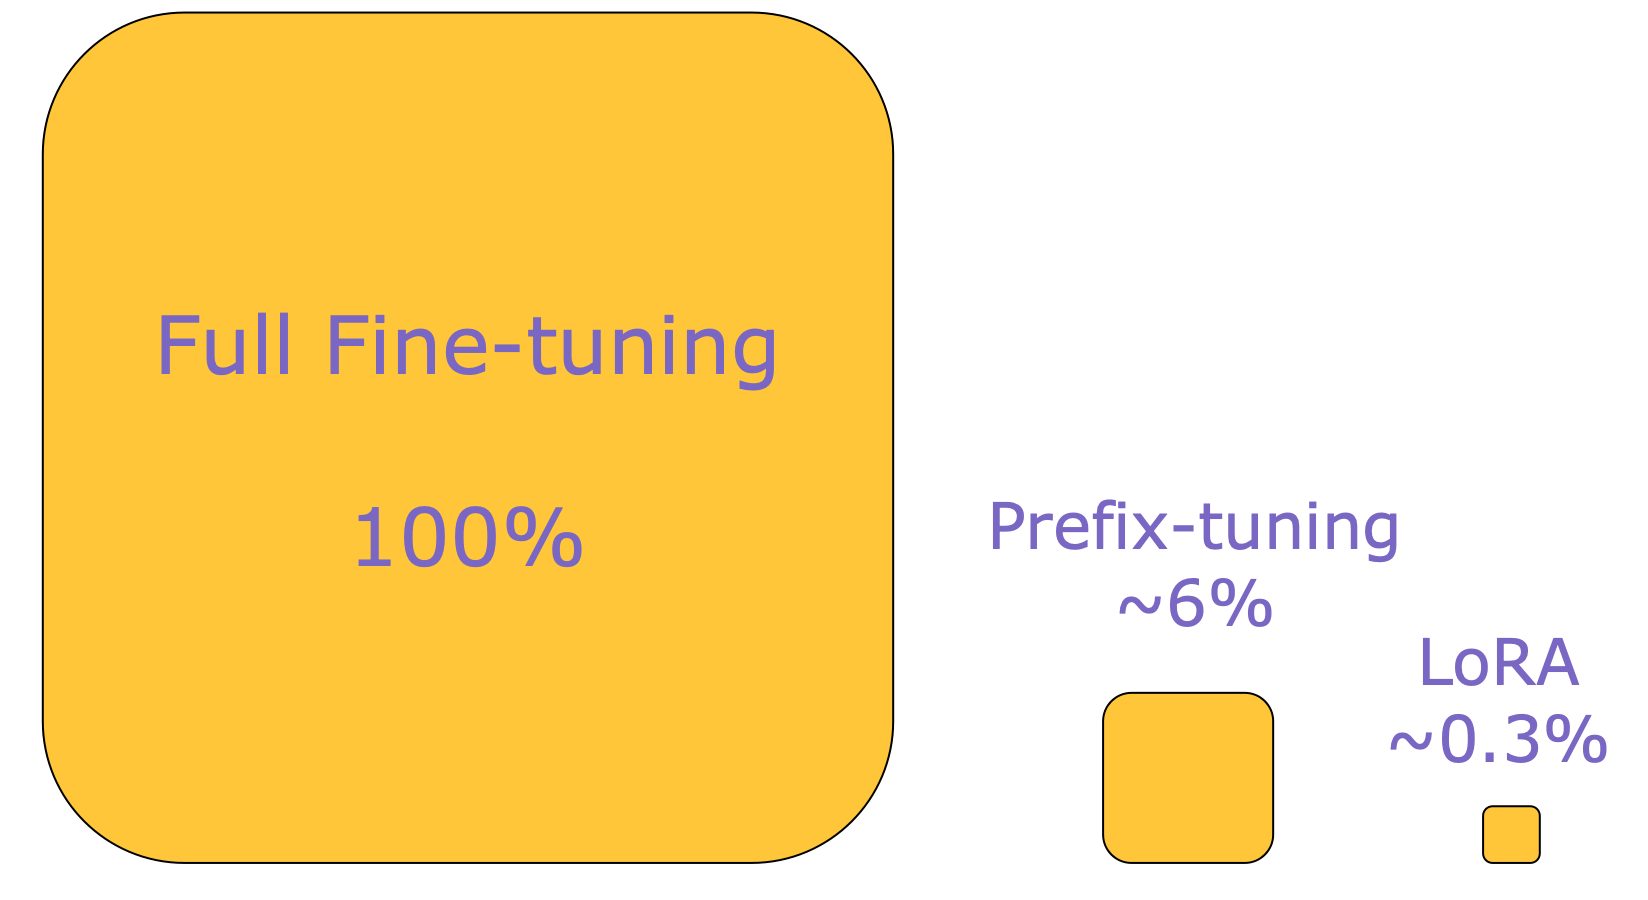
\includegraphics[width=0.6\textwidth]{fig/param-compare.png}
    % \caption{ROUGE-L scores of mT5$_{\text{BASE}}$.}
    \end{figure}

 \begin{block}{Experimental Setting}

    \textbf{Dataset: XL-Sum}, a large-scale multilingual abstractive summarization dataset containing news articles from BBC.
    We experimented on 11 languages containing both high- and low-resource ones: Arabic, Burmese, Chinese (Simplified), English, French, Hindi, Japanese, Korean, Russian, Spanish, and Turkish.

    \begin{table}
      \centering
      % \small
      \scalebox{0.8}{
      \begin{tabular}{lrrrrrrrrrrr}
        \hline
        \textbf{Lang.}   & ar     & my    & zh     & en      & fr     & hi     & ja    & ko    & ru     & es     & tr     \\ \hline
        \textbf{\#Train} & 37,519 & 4,569 & 37,360 & 306,522 & 8,697  & 70,777 & 7,113 & 4,407 & 62,243 & 38,110 & 27,176 \\
        \textbf{\#Dev}   & 4,689  & 570   & 4,670  & 11,535  & 1,086  & 8,847  & 889   & 550   & 7,780  & 4,763  & 3,397  \\
        \textbf{\#Test}  & 4,689  & 570   & 4,670  & 11,535  & 1,086  & 8,847  & 889   & 550   & 7,780  & 4,763  & 3,397  \\
        \textbf{\#Total} & 46,897 & 5,709 & 46,700 & 329,592 & 10,869 & 88,471 & 8,891 & 5,507 & 77,803 & 47,636 & 33,970 \\ \hline
      \end{tabular}}
      % \caption{XL-Sum dataset.}
    \end{table}

    \textbf{Models:} \textbf{mBART}$_{\textbf{LARGE}}$ and \textbf{mT5}$_{\textbf{BASE}}$. We compare full fine-tuning (FT), prefix-tuning (PT) with prefix length 100, and LoRA with rank 16.


  \end{block}

  % \begin{block}{Experiments}
  %   \lipsum[1]
  % \end{block}

  \begin{block}{Results}
    \begin{figure}
    \centering
    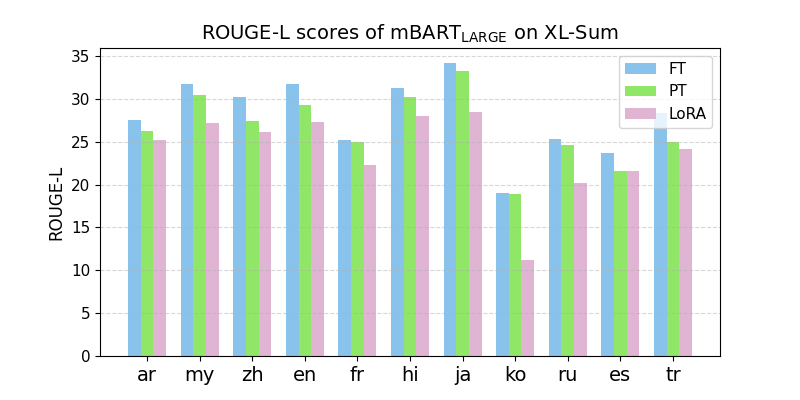
\includegraphics[width=\textwidth]{fig/mbart-result.png}
    % \caption{ROUGE-L scores of mBART$_{\text{LARGE}}$.}
    \end{figure}

    \begin{figure}
    \centering
    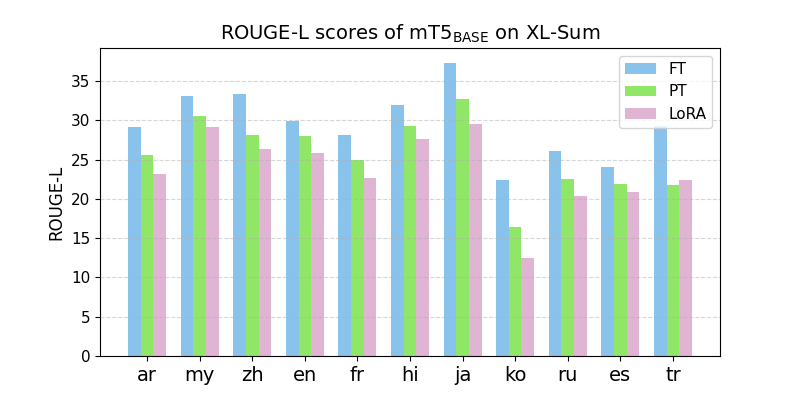
\includegraphics[width=\textwidth]{fig/mt5-result.png}
    % \caption{ROUGE-L scores of mT5$_{\text{BASE}}$.}
    \end{figure}
  \end{block}

\end{column}

\separatorcolumn

\begin{column}{\colwidth}

  % \begin{block}{Figure}
    % \begin{figure}
    %   \centering
    %   \begin{tikzpicture}[scale=2]
    %     \begin{axis}[
    %         scale only axis,
    %         no markers,
    %         domain=0:2*pi,
    %         samples=100,
    %         axis lines=center,
    %         axis line style={-},
    %         ticks=none]
    %       \addplot[red] {sin(deg(x))};
    %       \addplot[blue] {cos(deg(x))};
    %     \end{axis}
    %   \end{tikzpicture}
    %   \caption{Another figure caption.}
    % \end{figure}
  % \end{block}

  \begin{block}{Further Investigation into Prefix-tuning}
    \heading{Impact of Prefix Length}

    Performance optimization requires careful tuning of prefix length, which varies significantly by language.
    A one-size-fits-all approach to prefix length can be ineffective for multilingual abstractive summarization.

    \begin{figure}
    \centering
    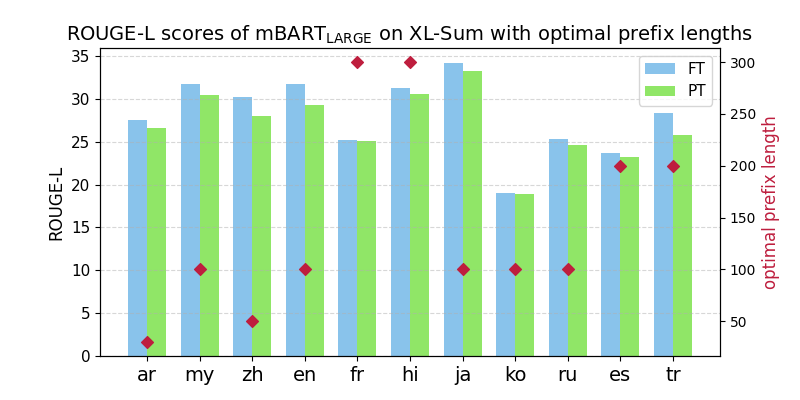
\includegraphics[width=\textwidth]{fig/mbart-opt-len.png}
    % \caption{ROUGE-L scores of mBART$_{\text{LARGE}}$ with optimal len.}
    \end{figure}


    \heading{Few-shot Performance}

    In few-shot scenarios with limited data available, prefix-tuning offers competitive and sometimes superior performance compared to full fine-tuning.
    This makes prefix-tuning an ideal choice for resource-constrained settings.
    % , further proving the efficiency and versatility of PEFT methods.

    \begin{figure}
    \centering
    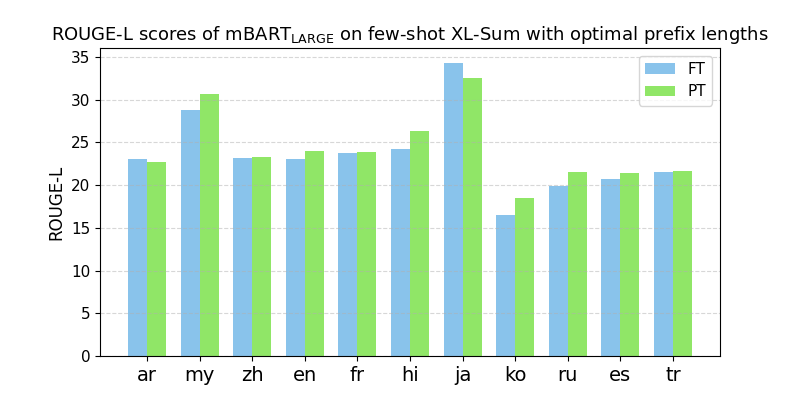
\includegraphics[width=\textwidth]{fig/mbart-few-shot.png}
    % \caption{ROUGE-L scores of mBART$_{\text{LARGE}}$ on few-shot.}
    \end{figure}
  \end{block}

  \begin{exampleblock}{Conclusion}
    \begin{enumerate}
      \item While PEFT methods can significantly reduce computational costs and memory usage, they exhibit a performance drop across languages when compared to full fine-tuning.
      \item We present the first comprehensive evaluation of PEFT methods for multilingual abstractive summarization, providing key insights into the balance between efficiency and performance and establishing benchmarks for future research.
      \item We include a detailed investigation into prefix-tuning, shedding light on its effectiveness under few-shot condition and providing valuable insights for optimizing its performance in multilingual settings.
    \end{enumerate}
  \end{exampleblock}

  \begin{block}{References}
    \nocite{*}
    \footnotesize{\bibliographystyle{abbrv}\bibliography{poster}}
  \end{block}

\end{column}
\separatorcolumn

% \begin{column}{\colwidth}
% \end{column}
% \separatorcolumn



\end{columns}
\end{frame}

\end{document}
